\documentclass[8pt,landscape,a4paper]{article}
\usepackage[margin=0.25in]{geometry}
\usepackage{multicol}
\usepackage{amsmath,amssymb}
\usepackage{enumitem}
\usepackage{titlesec}
\usepackage{xcolor}

\usepackage{graphicx}
\usepackage{fancyhdr}
\usepackage{geometry}
\usepackage{titlesec}
\usepackage{bm}
\usepackage[nolist]{acronym}
\usepackage[most]{tcolorbox}

% Reduce spacing
\setlength{\parindent}{0pt}
\setlength{\parskip}{0.5pt}
\setlength{\itemsep}{0pt}
\setlength{\parsep}{0pt}
\setlength{\topsep}{0pt}

% Section formatting
\titleformat{\section}{\normalfont\fontsize{10}{11}\bfseries\color{blue}}{\thesection}{0.5em}{}
\titleformat{\subsection}{\normalfont\fontsize{9}{10}\bfseries\color{teal}}{\thesubsection}{0.3em}{}
\titlespacing*{\section}{0pt}{1.2em}{0pt}
\titlespacing*{\subsection}{0pt}{0.7em}{0pt}

\begin{document}
\begin{multicols*}{3}

\section{Rational Agents}
\textbf{Agent:} Perceives via sensors, acts via actuators\\
\textbf{Rational:} Maximizes expected performance given percepts and knowledge ($\neq$ omniscient)\\
\textbf{Most challenging env:} Partially observable, nondeterministic, strategic, dynamic, continuous, multi-agent

\section{Search Fundamentals}
\textbf{Problem:} State space, initial state, actions, goal test, path costs\\
\textbf{Solution:} Action sequence from initial $\rightarrow$ goal state

\subsection{Search Criteria}
\textbf{Complete:} Finds solution if exists\\
\textbf{Optimal:} Lowest path cost\\
\textbf{Complexity:} $b$ (branching), $d$ (goal depth), $m$ (max depth)

\subsection{Uninformed Search}
\textbf{BFS:} layer by layer\\
\textbf{UCS:} Priority queue by path cost to node $n$: $g(n)$\\
\textbf{DFS:} deepest node first\\
\textbf{IDS:} DFS with increasing depth limits\\
\textbf{Bidirectional:} Forward+backward search

\section{CSPs}
\textbf{Variables:} $\{x_1,\ldots,x_n\}$, \textbf{Domains:} $\{dom_1,\ldots,dom_n\}$, \textbf{Constraints:} Allowable value combinations\\
\textbf{Solution:} Complete value assignment

\subsection{Backtracking Heuristics}
\textbf{Most-Constrained Var:} Fewest remaining values, red. $b$\\
\textbf{Most-Constraining Var:} Most constraints on unassigned, tie-breaker for (1)\\
\textbf{Least-Constraining Value:} Prefer value that rules out fewest choices for neighbors

\subsection{Inference}
\textbf{Forward Checking:} Delete inconsistent neighbor values, backtrack if any variables domain becomes empty\\
\textbf{Arc Consistency (AC-3):} $\forall x\in X, \exists y\in Y$ satisfying constraint, $O(d^3n^2)$, NP-hard

\subsection{Exploiting Structure}
\textbf{Disconn. components} of contraint graph can be solved independantly\\
\textbf{Tree CSPs:} $O(nd^2)$ with topological node order which enforces arc consistency (value assign. from root) (Almost-TCSPs: cutset conditioning (break loops in graph) and tree decomposition (connected subproblems organized as tree))

\section{Informed Search}
\textbf{Heuristic} $h(n)$ estimates cheapest cost to goal from node $n$\\
\textbf{Consistent} iff it is less than or equal to the actual cost of action a (overly optimistic) (implies admissibility)

\subsection{Best-First Variants}
\textbf{Greedy:} $f(n) = h(n)$, fast but incomplete/non-optimal\\
\textbf{A*:} $f(n) = g(n) + h(n)$ (UCS + Best-First)\\
- Complete/optimal if $h$ admissible: $h(n) \leq h^*(n)$\\
- Graph-search optimal if $h$ consistent, $h(s) - h(s')\leq c(a)$\\
- Exponential space complexity\\
\textbf{IDA*:} f-cost cutoff, memory efficient

\subsection{Local Search (if goal path irrelevant)}
\textbf{Hill-climbing:} Move to best neighbor state, issues: local maxima/plateaus/ridges\\
\textbf{Simulated annealing:} Accept bad moves with decreasing probability (temperature $T$)\\
\textbf{Genetic algorithms:} Population evolution: fitness func for individuals, selection, crossover, mutation

\section{Games}
\textbf{Game:} Initial state, operators (legal moves), terminal test, utility function (outcome of game)\\
\textbf{Properties:} States fully accessible, contingency problem, huge state space

\subsection{Minimax}
DFS game tree, MAX maximizes, MIN minimizes utility\\
Use evaluation function for non-terminals (prefer quiescent positions) to avoid horizon effect

\subsection{Alpha-Beta Pruning}
$\alpha$: best MAX value, $\beta$: best MIN value so far\\
Prune when $\alpha \geq \beta$ (both MIN and MAX),
Best case: $b \rightarrow \sqrt{b}$ (depends on move ordering)

\subsection{Chance Games}
Add chance nodes: value = $\sum P(\text{outcome}) \times \text{value}(\text{outcome})$

\section{Propositional Logic}
\textbf{Syntax:} Literals, clauses (disjunctions), \textbf{Semantics:} Truth interpretations
\textbf{Entailment:} KB $\models \alpha$ if $\alpha$ true in all KB models

\subsection{CNF Conversion}
1. Eliminate $\Rightarrow, \Leftrightarrow$: $\alpha \Rightarrow \beta$ becomes $(\neg\alpha \vee \beta)$\\
2. Move $\neg$ inward: $\neg(\alpha \wedge \beta)$ becomes $(\neg\alpha \vee \neg\beta)$  \\
3. Distribute $\vee$ over $\wedge$: $(\alpha\wedge\beta)\vee\gamma$ becomes $(\alpha\vee\gamma)\wedge(\beta\vee\gamma)$

\textbf{CNF:} $\bigwedge_{i=1}^n\left(\bigvee_{j=1}^{m_i} l_{i,j}\right)$, \textbf{DNF:} $\bigvee_{i=1}^n\left(\bigwedge_{j=1}^{m_i} l_{i,j}\right)$

\subsection{Resolution (derive formulae from KB)}
\textbf{Goal:} Prove KB $\models \alpha$ by showing KB $\cup \{\neg\alpha\}$ unsatisfiable\\
\textbf{Req:} All sentences in CNF\\
\textbf{Rule:} From $C_1 \cup \{l\}, C_2 \cup \{\neg l\}$ derive resolvent $C_1 \cup C_2$
Empty clause $\square$ proves unsatisfiability

\section{Boolean Satisfiability Problem (SAT)}
\textbf{Goal:} Find satisfying assignment (model) for CNF formula or prove none exists.

\subsection{DPLL}
Given a set of clauses $\Delta$ over a set of variables $\Sigma$:\\
1. If $\Delta = \emptyset$ return ``satisfiable''\\
2. If $\square \in \Delta$ return ``unsatisfiable''\\  
3. Unit propagation: assign unit clause literals, recurse\\
4. Split: try both values for unassigned variable, recurse

\subsection{CDCL}
Enhances DPLL with conflict analysis, clause learning and backjumping.

% \section{First-Order Predicate Logic}
% \textbf{Extensions:} Quantifiers ($\forall,\exists$), variables, functions, predicates
% \textbf{Terms:} Constants, variables, function applications
% \textbf{Atomic formulas:} $P(t_1,\ldots,t_n)$ or $t_1 = t_2$

% \subsection{Semantics}
% \textbf{Interpretation:} Domain $D$ + mappings for constants/functions/predicates
% \textbf{Closed formulas:} No free variables (sentences)

% \subsection{Propositionalization}
% For finite domains: replace quantifiers with conjunctions/disjunctions
% $\forall x \phi$ becomes $\phi[x/c_1] \wedge \phi[x/c_2] \wedge \ldots$
% $\exists x \phi$ becomes $\phi[x/c_1] \vee \phi[x/c_2] \vee \ldots$

\section{Action Planning}
\textbf{Goal:} Find action sequence to achieve goals.

\subsection{STRIPS}
\textbf{States:} Sets of true propositions (closed world assumption)\\
\textbf{Actions:} Preconditions + effects (add/delete lists)\\
\textbf{Planning task:} $\langle S,O,I,G\rangle$ (states, operators, initial, goal)

\subsection{PDDL}
Standard planning language, extends STRIPS with typing, conditional effects, numerical resources

\subsection{Algorithms}
\textbf{Progression:} Forward search from initial state\\
\textbf{Regression:} Backward search from goal

\section{Probability / Decisions}
\textbf{Prior:} $P(A)$, \textbf{Posterior:} $P(A|B)$\\
\textbf{Product rule:} $P(A \wedge B) = P(A|B)P(B)$\\
\textbf{Independence:} $P(a|b) = P(a)$ iff $P(a \wedge b) = P(a)P(b)$\\
\textbf{Bayes' Rule:}
$$P(\text{cause}|\text{effect}) = \frac{P(\text{effect}|\text{cause})P(\text{cause})}{P(\text{effect})}$$

\subsection{Bayesian Networks}
\textbf{Structure:} Directed Acyclic Graph, nodes = variables, edges = dependencies\\
\textbf{Joint distribution:} $P(x_1,\ldots,x_n) = \prod_{i=1}^n P(x_i|\text{parents}(x_i))$\\
\textbf{Inference:} Generally NP-hard, $O(2^n)$. Linear for polytrees.\\
\textbf{Conditional Independence:} Node independent of non-descendants given parents

\section{(Action) Decision Theory}
\textbf{Utility:} $U(S)$ assigns values to states\\
\textbf{Axioms:} Orderability, Transitivity, Continuity\\
\textbf{MEU:} $EU(A|E) = \sum_i P(\text{Result}(A)=i|\text{Do}(A),E)U(i)$ (rational agent maximizes MEU)

\subsection{MDPs}
\textbf{Components:} States $S$, actions $A$, transitions $P(s'|s,a)$, rewards $R(s)$\\
\textbf{Policy:} $\pi(s)$ maps states $\rightarrow$ actions (goal: find $\pi*$)

\subsection{Bellman Equation}
$U(s) = R(s) + \gamma \max_a \sum_{s'} P(s'|s,a)U(s')$ \\

$\pi(s) = \arg\max_a \sum_{s'} P(s'|s,a)U(s')$

\subsection{Algorithms}
\textbf{Value iteration:} $U'(s) \leftarrow R(s) + \gamma \max_a \sum_{s'} P(s'|s,a)U(s')$
\textbf{Policy iteration:} Alternate evaluation + improvement

\section{Machine Learning}
\textbf{Ockhams razor:} Choose simplest hypothesis consistent with the data

\subsection{Decision Trees}
\textbf{Algorithm:} Greedy divide-and-conquer\\
1. Same class $\rightarrow$ leaf\\
2. Select best attribute (max info gain)\\
3. Recurse\\
\textbf{ - Entropy:} $I(P(y_1),\ldots,P(y_n)) = \sum_{i=1}^n -P(y_i)\log_2 P(y_i)$\\
\textbf{ - Evaluation:} Separate training/test sets

\section{Deep Learning}
Multiple layers learn feature hierarchies

\subsection{MLPs}
\textbf{Structure:} Input, hidden, output layers
\textbf{Training:} Minimize loss with SGD + backpropagation

\columnbreak

\section{Quick Reference}

\subsection{Search Complexities}

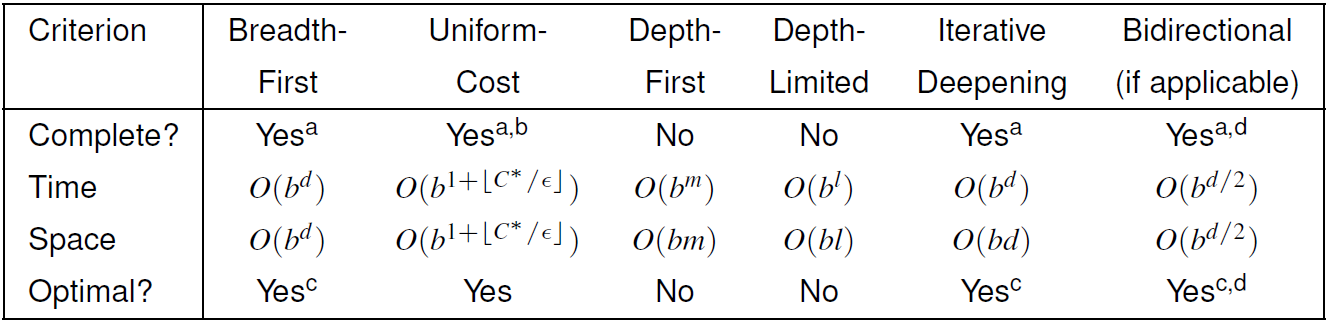
\includegraphics[width=\columnwidth]{searches1.png}
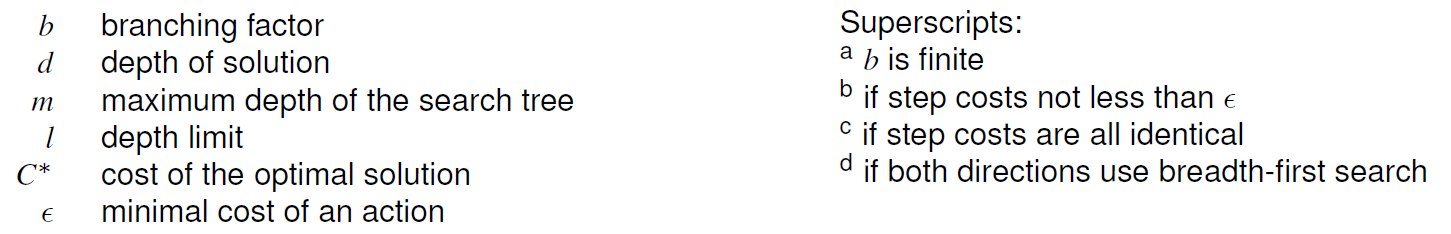
\includegraphics[width=\columnwidth]{searches2.png}

\subsection{Probability Rules}
$P(A \cup B) = P(A) + P(B) - P(A \cap B)$\\
$P(A|B) = \frac{P(A \cap B)}{P(B)}$ if $P(B) > 0$

\subsection{Logic Equivalences}
$\neg(A \wedge B) \equiv (\neg A \vee \neg B)$ (De Morgan)\\
$\neg(A \vee B) \equiv (\neg A \wedge \neg B)$ (De Morgan)\\
$(A \Rightarrow B) \equiv (\neg A \vee B)$\\
$(A \Leftrightarrow B) \equiv ((A \Rightarrow B) \wedge (B \Rightarrow A))$

\subsection{AC-3 Step-by-Step}
For each arc $(X_i, X_j)$: Remove values from $dom(X_i)$ that have no supporting value in $dom(X_j)$. If domain becomes empty, return inconsistent.

\subsection{CNF Conversion Examples}
$\phi \Leftrightarrow \psi \equiv (\phi \Rightarrow \psi) \wedge (\psi \Rightarrow \phi)$
$\equiv (\neg\phi \vee \psi) \wedge (\neg\psi \vee \phi)$

\subsection{Resolution Steps}
To prove $KB \models \alpha$ show that $K\cup\left\{\neg\alpha\right\}\models\bot $:\\
1. Add $\neg\alpha$ to KB\\
2. Convert all to CNF clauses\\
3. Apply resolution rule until $\square$ derived\\
4. If $\square$ found $\Rightarrow$ KB $\models \alpha$

\subsection{MDP Value Update}
$U^{t+1}(s) = R(s) + \gamma \max_a \sum_{s'} P(s'|s,a) U^t(s')$

\subsection{MDP Policy Improvement}
1. Policy evaluation, given policy $\pi_t$ calc. utilities $U_t=U^{\pi_t}$\\
2. Policy improvement $$\pi_{t+1}(s)=\textrm{argmax}_a\sum_{s'}P(s'|s,a)U_t(s')$$


\subsection{Probability Calculations}
$P(A \cup B) = P(A) + P(B) - P(A \cap B)$\\
$P(A|B) = \frac{P(A \cap B)}{P(B)}$\\
If mutually exclusive: $P(A \cap B) = 0$\\
If independent: $P(A|B) = P(A)$

\subsection{Information Gain Calculation}
$Gain(A) = Entropy(S) - \sum_{v} \frac{|S_v|}{|S|} Entropy(S_v)$

where $S_v$ = subset with attribute $A = v$

\textbf{Entropy:} $H(S) = -\sum_i p_i \log_2 p_i$

\subsection{Alpha-Beta Pruning Rules}
Initialize root with $\alpha=-\inf$, $\beta=\inf$\\
Prune if $\beta \leq \alpha$ \\
Update: $\alpha = \max(\alpha, value)$ at MAX\\
Update: $\beta = \min(\beta, value)$ at MIN

\subsection{CSP Arc Consistency}
Arc $X \rightarrow Y$ consistent if:
$\forall x \in D_X, \exists y \in D_Y$ such that $(x,y)$ satisfies constraint

\subsection{Minimax with Chance}
Expected value at chance nodes:
$V = \sum P(outcome_i) \times V(child_i)$

\subsection{A* Completeness}
Finite state space, non-negative edge costs

\subsection{Misc}
If two events A and B are unconditionally independent, they may not be conditionally independent given another event C.\\

If two DTs are equally accurate, the one with fewer nodes is preferrable since it is less prone to overfitting.\\

ML: Manual feature engineering, simpler models, perform well on structured data and simpler problems, requires less computational power\\

DL: Automatically learns features from data, can handle large complex datasets by learning hierarchical features and using deep architectures, requires a lot more computational power
\end{multicols*}
\end{document}